\paragraph{1. Library toevoegen}
Eerst moet de Notifee library aan de root van ons project worden toegevoegd. 
Deze wordt toegevoegd met volgende commando:
\begin{minted}{bash}
npm install --save @notifee/react-native
\end{minted}

\paragraph{2. Toestemming vragen \& channel aanmaken}
Nog voor een notificatie kan getoond worden moet er eerst toestemming worden gevraagd. 
Aangezien dit bij React Native niet automatisch gebeurt zoals bij Android moet de 
toestemming programmatisch gevraagd worden. Daarnaast zal ook een channel moeten aangemaakt worden.
Net zoals bij Android maakt het niet uit wanneer dit gebeurt maar het moet wel gebeuren 
voor dat er notificaties worden gestuurd. Dus best zo vroeg mogelijk in de applicatie.
\begin{minted}{javascript}
export const notificationsSetup = async () => {
  const PERMISSION = await notifee.requestPermission();

  if(PERMISSION.authorizationStatus === AuthorizationStatus.DENIED) {
    return;
  }

  await notifee.createChannel({
    id: 'bachproef',
    name: 'BachproefNotificaties',
  });
}

\end{minted}

\paragraph{3. Notificatie aanmaken}
Bij React Native worden notificaties direct getoond bij het maken ervan. Net zoals bij Android 
wordt er een naam, description, channelId en optioneel een icon (default ic\_launcher) meegegeven. 
\begin{minted}{javascript}
export const createNotification = async (title: string, body: string) => {
  await notifee.displayNotification({
    title,
    body,
    android: {
      channelId: 'bachproef',
      pressAction: {
        id: 'default',
      },
    },
  });
}
\end{minted}

\paragraph{4. Applicatie maken}
Net zoals bij native zal de applicatie bestaan 
uit twee \textbf{<TextInput/>} componenten voor een titel en beschijving van de notificatie en tot slot een 
\textbf{<Button/>} om de notificatie te triggeren. Als de knop wordt ingedrukt dan wordt de 
\textbf{createNotification} methode aangeroepen en wordt de waarde van de inputs meegegeven.
\begin{figure}[H]
  \centering
  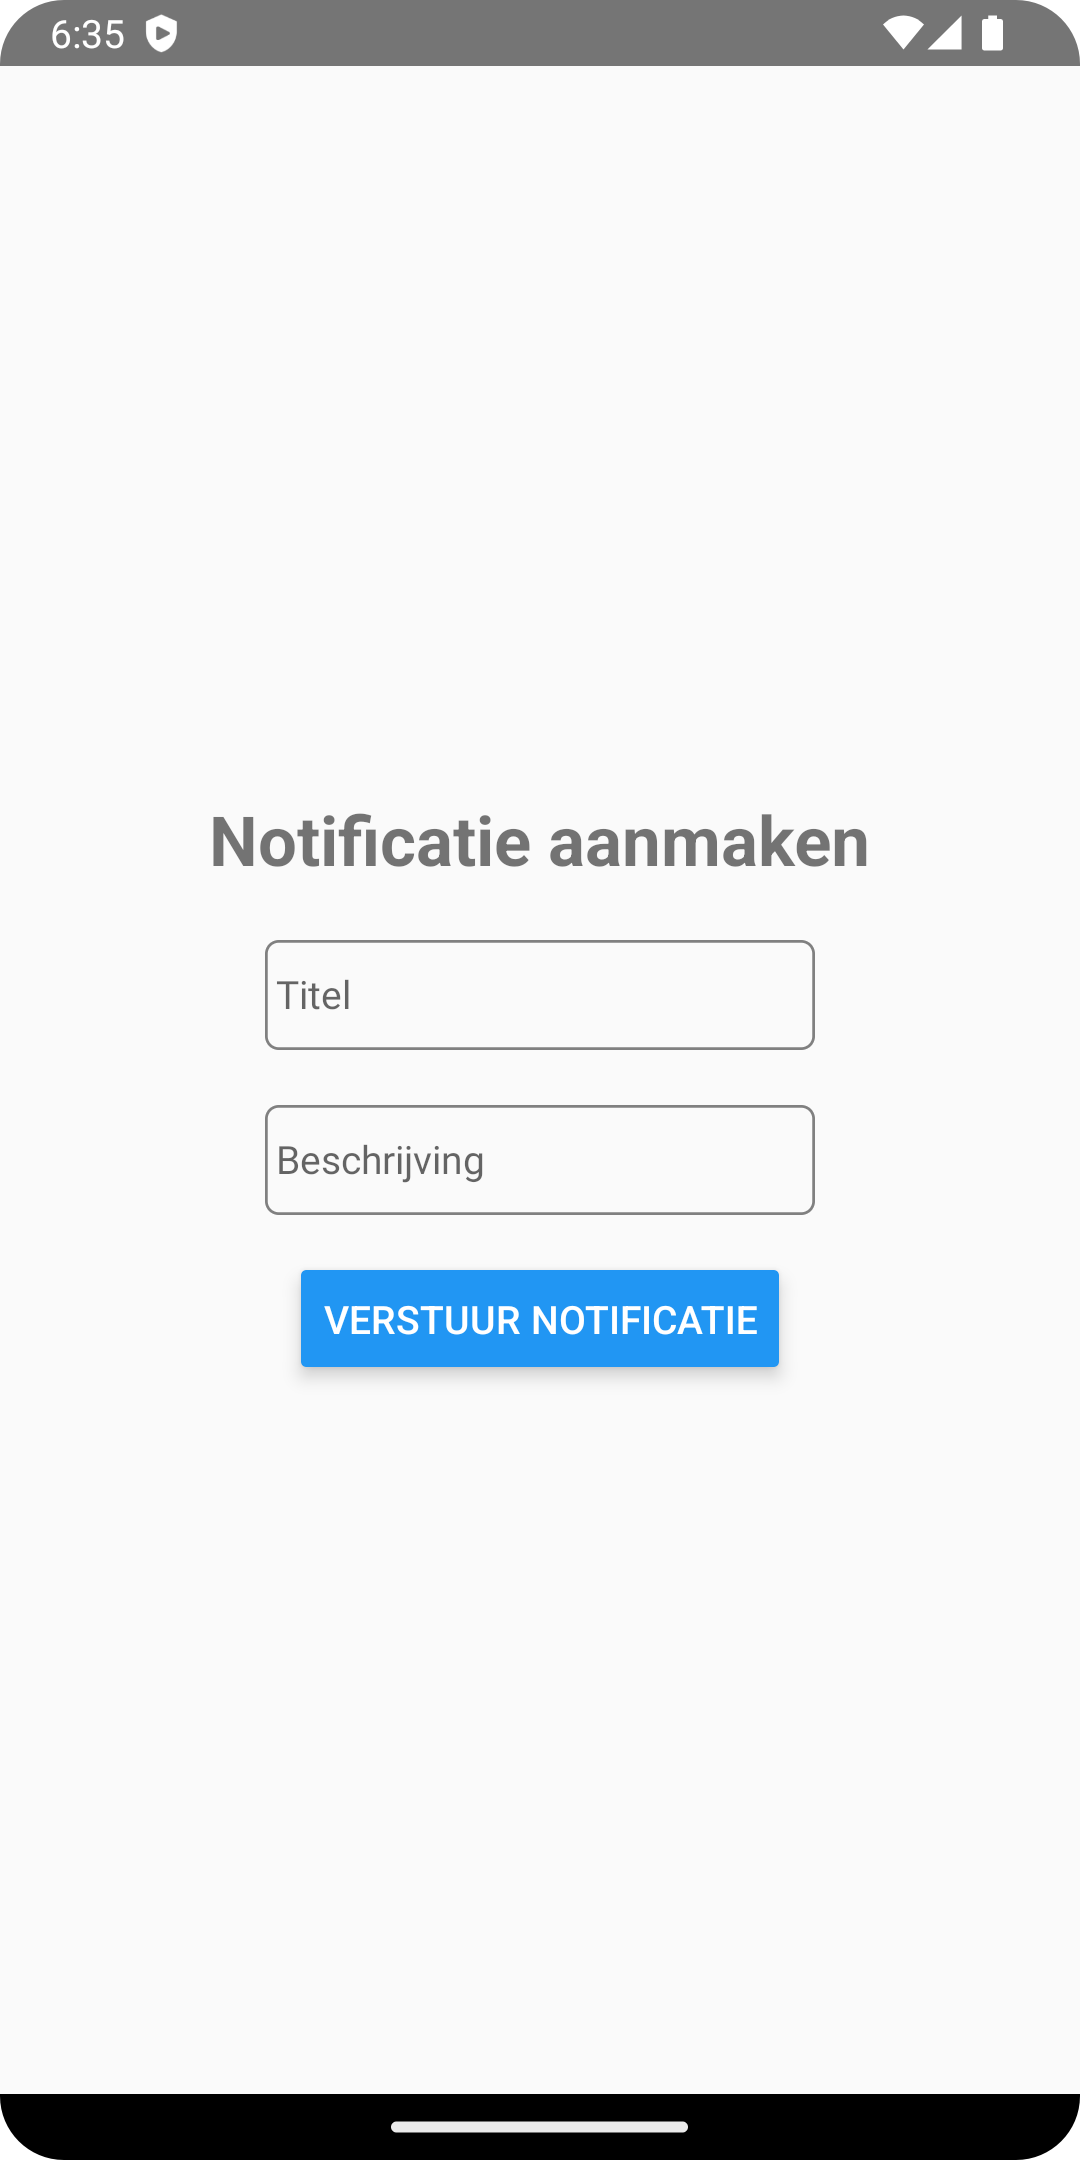
\includegraphics[height=0.5\textheight]{notificaties_layoutcross.png}
  \caption{Layout van applicatie voor notificaties te sturen bij React Native.}
\end{figure}